% Modeled after the following
% A simple Tree
% Author: Stefan Kottwitz
% https://www.packtpub.com/hardware-and-creative/latex-cookbook
\documentclass[border=10pt]{standalone}
\usepackage{tikz}
\begin{document}
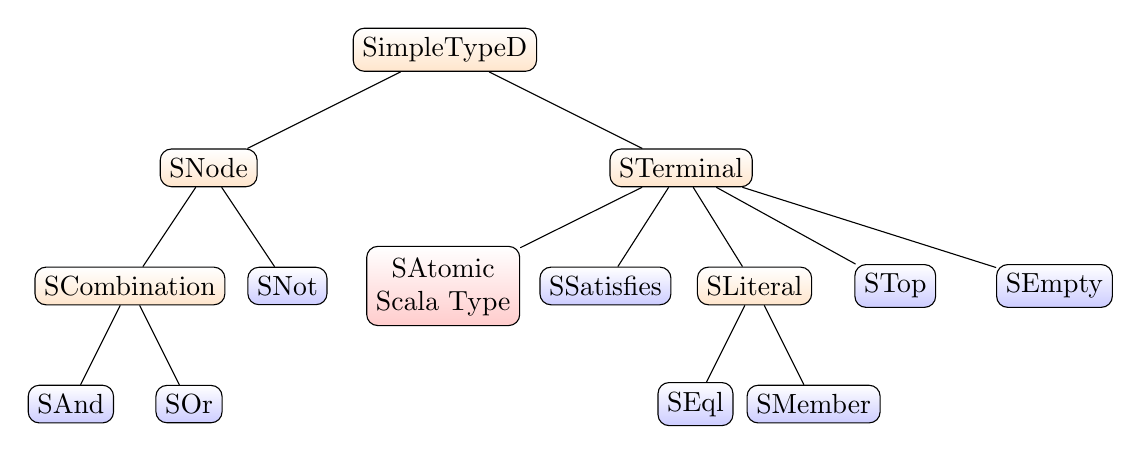
\begin{tikzpicture}[sibling distance=10em,
  every node/.style = {shape=rectangle, rounded corners,
    draw, align=center,
    top color=white, bottom color=blue!20}]]
    \tikzstyle{level 1}=[sibling distance=60mm]
    \tikzstyle{level 2}=[sibling distance=20mm]
    \tikzstyle{level 3}=[sibling distance=15mm]
  \node [bottom color=orange!20] {SimpleTypeD}
    child { node [bottom color=orange!20] {SNode}
      child { node [bottom color=orange!20] {SCombination} 
        child { node {SAnd} }
        child { node {SOr} } }
      child { node {SNot} } }
    child { node [bottom color=orange!20] {STerminal}
      child { node [text height=20pt, right=0mm, top color=white, bottom color=red!20] {SAtomic\\Scala Type } }
      child { node [right=2mm] {SSatisfies} }
      child { node [right=2mm] [bottom color=orange!20] {SLiteral}
        child { node {SEql} }
        child { node {SMember} } }
      child { node [right=2mm] {STop} }
      child { node [right=0mm] {SEmpty} } } ;
\end{tikzpicture}
\end{document}
